\documentclass{IEEEtran}
\usepackage{csquotes}
\usepackage{url}
\usepackage{graphicx}
\usepackage{caption}
\usepackage{xcolor,colortbl}
\usepackage{textcomp} 
\usepackage{listings}

\newcommand{\mc}[2]{\multicolumn{#1}{c}{#2}}
\definecolor{Gray}{gray}{0.95}
\definecolor{LightCyan}{rgb}{0.88,1,1}

\newcolumntype{a}{>{\columncolor{Gray}}l}
\newcolumntype{b}{>{\columncolor{white}}c}

\graphicspath{{./img/}}

\begin{document}

\title{CSE 578: Data Visualization}
\author{Claudio Rodriguez Rodriguez}
\maketitle

\section{Introduction}

The goal of the project is to create Visualizations that would help UVW College create Marketing Profiles. The Dataset used in the project comes from the 1994 Census Bureau Database extracted by Barry Becker \cite{cse578:kohaviNbtree}. UVW College is also interested in building a model based on the data, and part of the goal is to show enough factors and relationships that would help UVW College tailor their product offerings. Rows have a classification label of $>50K$ or $<=50K$ in Salary.  

The team started with a Jupyter Notebook to load the data, with some example queries so that every team member could quickly catch up. This notebook allowed some standardization of the tools to use, and some team members with fewer Pandas experience to start working immediately.

We built all visualizations using Python, with plots using Matplotlib or Plotly, Pandas for Data Retrieval, and SHAP for replicating Census Income Classification done by Scott Lundberg \cite{cse578:censusIncomeClassificationLightgbm}. The entire team assembled a System Documentation Report and an Executive Report to present the results of researching the data. 

While developing the research, the team had to discuss slowly on the ethical implications of the findings. We found value in our SHAP analysis as it showed a heavy bias toward the most prominent sample in the dataset. SHAP solved answers like "What is the combination of Attributes most likely to earn $>50K$?", but without a breakdown of each Attribute compared to the Salary Label, the algorithm can only reflect what the data is showing \cite{slack2019fooling}, regarding of the underlying biases within it. For example, we have twice the samples for males than females. It's essential to understand SHAP's role in the study to explain its findings to our stakeholders adequately, and the author provides an article to help explain how to use the algorithm to discover fairness in the data \cite{ExplainingMeasuresofFairnessAvoidt}. 

We attempt to show all possible combinations of Attributes in the dataset to transmit each potential profile's specific behavior for UVW College. Not all attributes show a strong correlation, showing little to no influence on the label class. 

\section{Description of Solution}


We started by developing a template that downloaded all the data and did some basic queries to level the field in the form of a Jupyter Notebook. Our queries were simple Selects, Group By, and Filter using Pandas. It wasn't possible to group the entire team, and communication via chat was not always reliable as each member were working professionals. 

Our second step was to develop questions for the data that would find different groups of people. We take our definition of marketing profile from \cite{perreault2002basic} as the lifestyle dimensions of the target audience, and limit it only to the demographics available in the Census data. 

We assume UVW College might have "incentives" to target different demographics from low income or low representation groups. Per Wilson and Carlsen \cite{wilson2016school}, we confirm that schools have various incentives to target different races and that colleges have intense competition in the marketing space, sometimes creating different "messages" for each demographic they are trying to attract.

Due to imbalanced numbers between male and female samples in the dataset, we proceeded to break each gender visualization as a first step. Similarly, we assume UVW College wants visualizations to observe all demographics to have their executives reach their conclusions on the data. 

We break down each attribute using both the Label Class Salary and the Sex attribute. We then proceed to use the following questions as our guide to discover relationships on the data:

\begin{itemize}
  \item What is the distribution of Education depending on the Country? 
  \item Any opportunities to help people in different marital status?
  \item Is there a correlation with hours worked and more salary? And would we be able to ensure that with a degree people would be able to work less?
  \item At what age do people start having College in their radar?
\end{itemize}

Based on figure~\ref{fig:EducationDistributionByCountryOfOrigin}, we can observe that the data doesn't show a lot of interest in College Education from people in which Native Country is the US.

\begin{figure}[!t]
  \centering
  \captionsetup{justification=centering}
  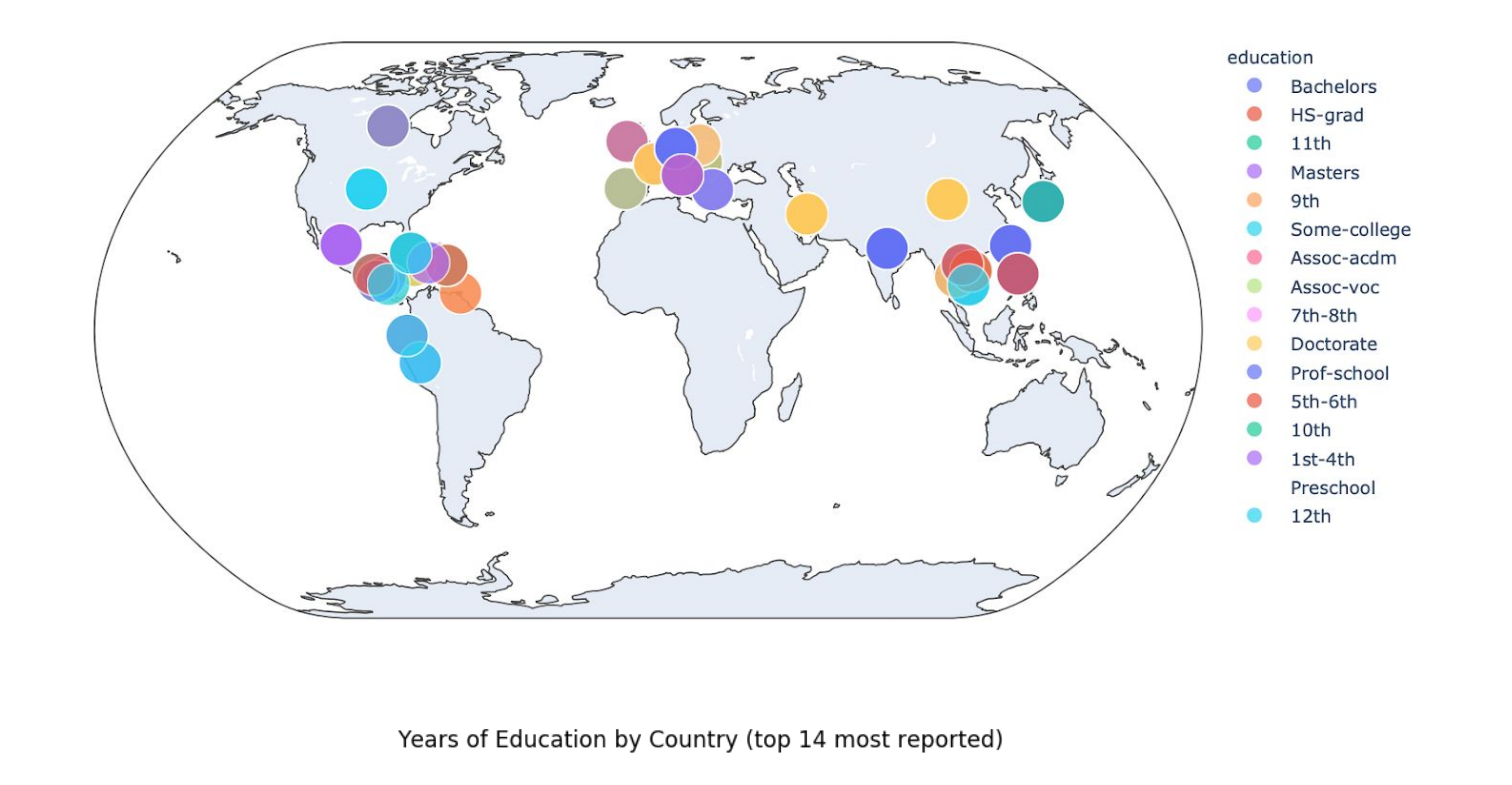
\includegraphics[width=0.5\textwidth]{EducationDistributionByCountryOfOrigin.png}%
  \caption{Education Distribution depending on Country of Origin}%
  \label{fig:EducationDistributionByCountryOfOrigin}%
\end{figure}

Figure~\ref{fig:DistributionOfIncomePerSexScatter} shows us the data distribution of Age vs. Entries in the dataset. We can observe there is a right skewness on the data, which we can correlate with people retiring the higher ages.

\begin{figure}[!t]
  \centering
  \captionsetup{justification=centering}
  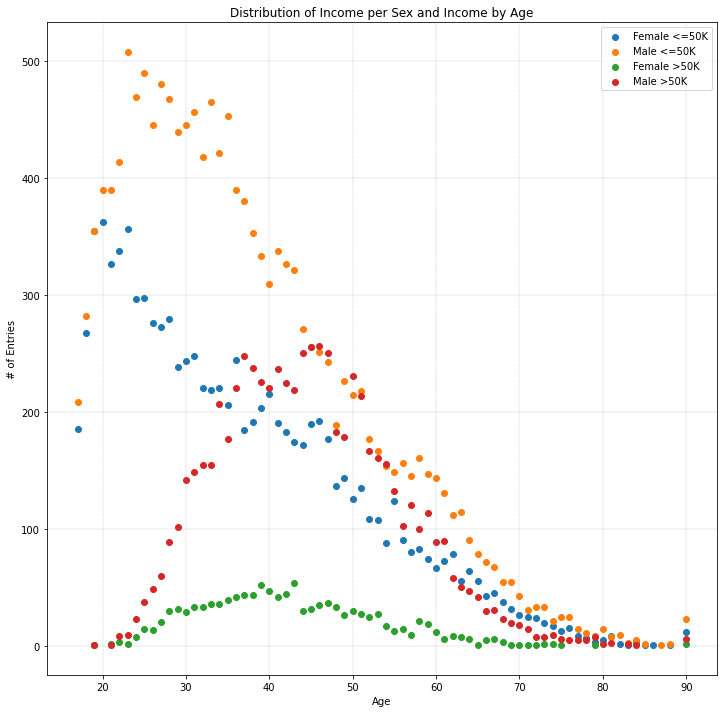
\includegraphics[width=0.5\textwidth]{DistributionOfIncomePerSexScatter.png}%
  \caption{Distribution of Entries by Salary and Sex}%
  \label{fig:DistributionOfIncomePerSexScatter}%
\end{figure}

We used Box Whisker Plot to observe outliers in the data and answer the question, "Is Higher Education Worth it?" Evidence proves that College education would net a positive, with a rising value of a college degree by 2014 at least \cite{leonhardt2014college}, even considering the increasing tuition costs \cite{daly2014still}. But in 2016, gains from going to College would range from $\$95,000$ to $\$275,000$ depending on the major\cite{webber2016college}, showing that it wasn't a definite conclusion. By 2019, breaking down groups by race showed a further decline in the returns of a bachelor's degree for White families, and other races seeing further weakening to the point that it adds very little value\cite{emmons2019college}. If we add to this factor a Global Pandemic that might make obtaining resources to pay for College unsustainable, UVW College could be facing a big challenge in phrasing their offerings as a net positive experience.

Using SHAP Analysis as an Explainable AI Tool, we could retrieve how each Attribute affected the label Class. Give the shape of the data SHAP results could lead to very misleading reports to Business. While \cite{slack2019fooling} leads us to conclude that we can manipulate SHAP to give unethical or biased results. These SHAP Weights can be observed in Table~\ref{table:ShapValues}. 


\begin{table}[!t]
  \centering
  \begin{tabular}{a | c}
    \hline
    Attribute & SHAP Importante \\
    \hline
    relationship	& $0.840923$ \\
    age	& $0.673732$ \\
    education-num	& $0.50265$ \\
    capital-gain	& $0.477472$ \\
    hours-per-week	& $0.326988$ \\
    marital-status	& $0.321257$ \\
    occupation	& $0.300844$ \\
    sex	& $0.235083$ \\
    capital-loss	& $0.141243$ \\
    fnlwgt	& $0.071476$ \\
    workclass	& $0.0534353$ \\
    race	& $0.0357368$ \\
    education	& $0.035535$ \\
    native-country	& $0.0169133$ \\ \hline
  \end{tabular}
  \caption{Higher weight means a higher change on the Label Class}%
  \label{table:ShapValues}%
\end{table}

We use the SHAP Weights to order the visualizations we want to retrieve from the data, leading us to correlations with Salary and Marital Status, Education Number by Race, Label Distribution depending on the existence of Capital Gains. 

\begin{figure}[!t]
  \centering
  \captionsetup{justification=centering}
  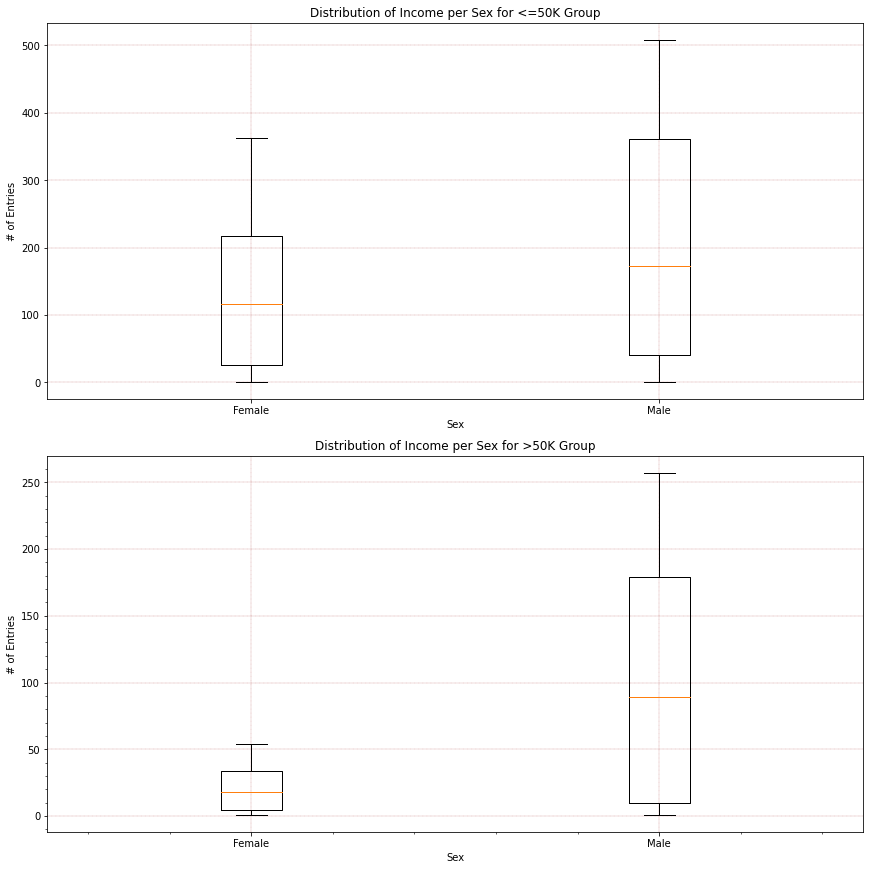
\includegraphics[width=0.5\textwidth]{DistributionOfIncomePerSex.png}%
  \caption{Distribution of Income Per Sex}%
  \label{fig:distributionOfIncomePerSex}%
\end{figure}

We also show the distribution of Income per Sex observed in Figure~\ref{fig:distributionOfIncomePerSex} and pair it with the conclusion of the question on higher education profitability. This finding leads us to investigate more into the education level of women in general. While the wage gap has been an essential topic of discussion with studies gathering and analyzing data from 1970-2010\cite{blau2017gender}, we have only recently started seeing that women tend to have a more significant blueprint than men in all majors\cite{hess_2019}. 

\section{Results}

To observe the conclusion to "Is Higher Education Worth it?" we created the visualizations in Figure~\ref{fig:DistrbutionOfEducationLevel} and Figure~\ref{fig:EducationByEthnicity}. These visualizations show that overall more Education leads to a higher salary, but each race has very different results. Keeping in mind that the data contains more samples for the White race, these plots should not be confused with the conclusion that the most prevalent race in the dataset has more Education.

\begin{figure}[!t]
  \centering
  \captionsetup{justification=centering}
  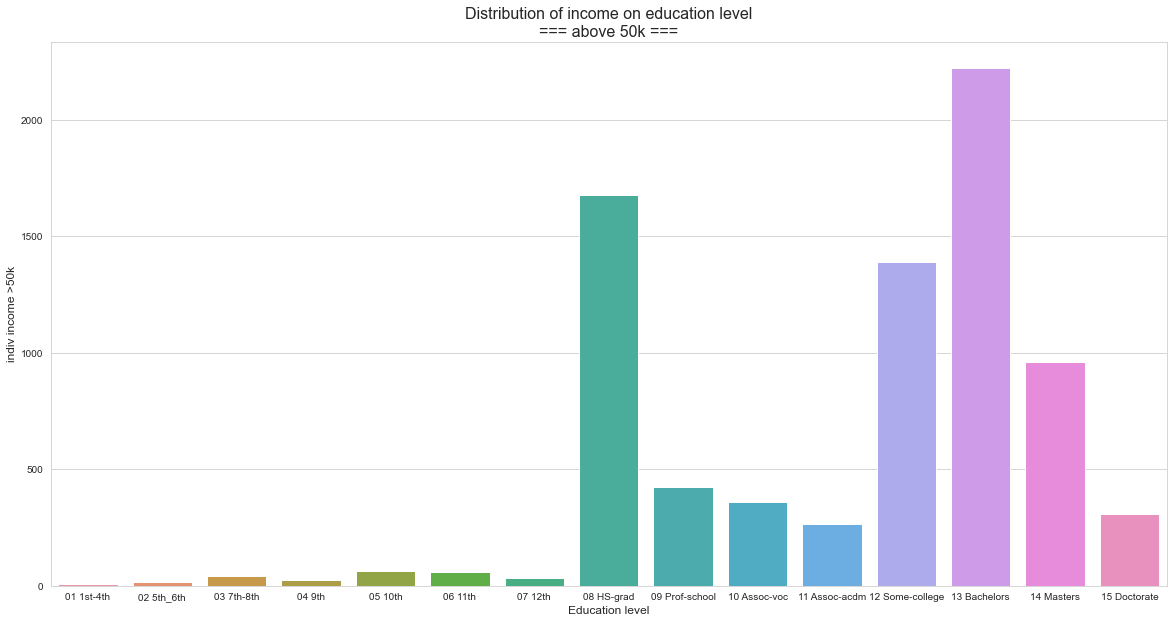
\includegraphics[width=0.5\textwidth]{EducationLevelVsSalary.png}%
  \caption{Education Level vs. Salary Distribution}%
  \label{fig:DistrbutionOfEducationLevel}%
\end{figure}

\begin{figure}[!t]
  \centering
  \captionsetup{justification=centering}
  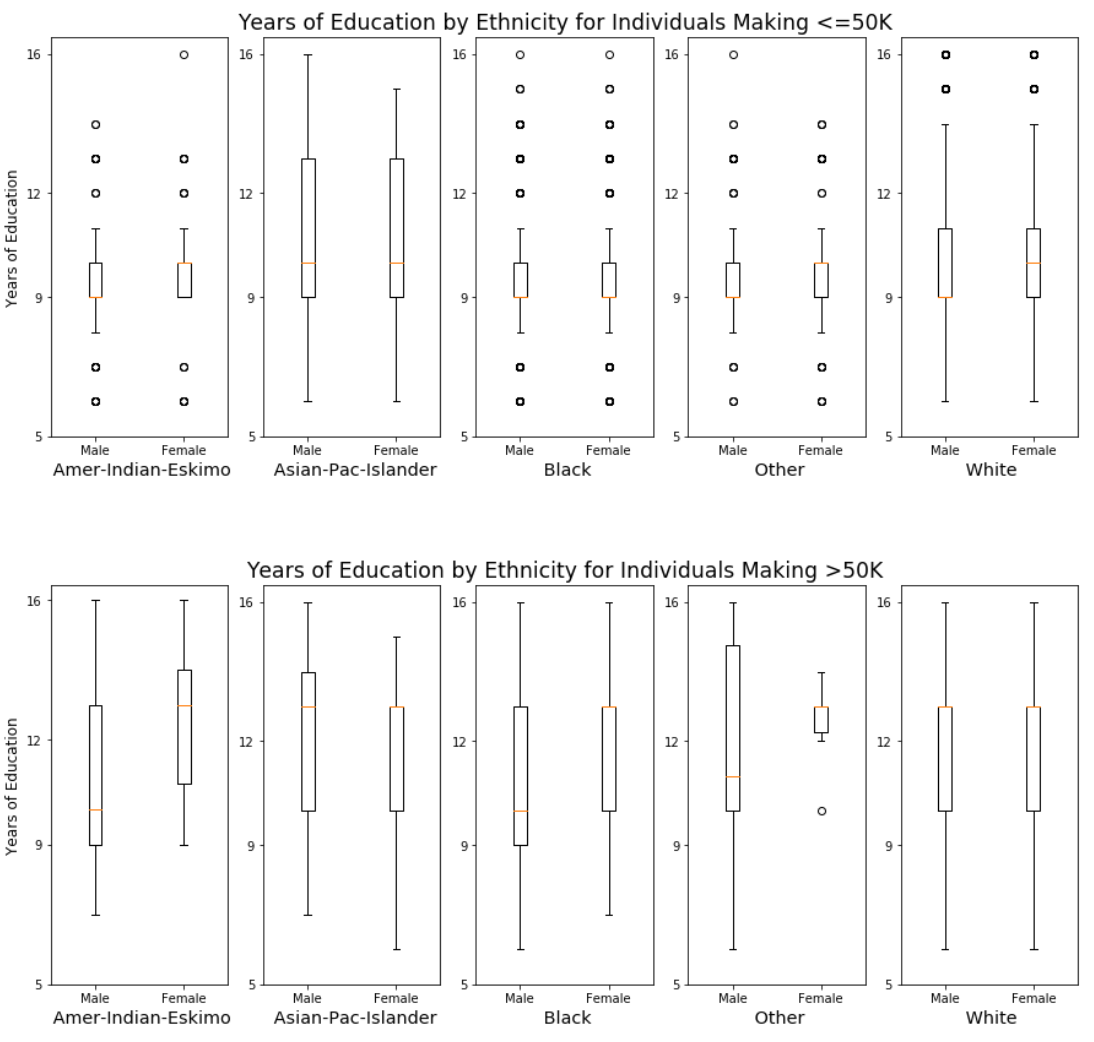
\includegraphics[width=0.5\textwidth]{YearsOfEducationByEthnicity.png}%
  \caption{Breaking Education by Ethnicity}%
  \label{fig:EducationByEthnicity}%
\end{figure}

One exciting finding was discovering that for people younger than 31, we can observe a higher degree of women obtaining Doctorates as long as they are not part of the Amer-Indian-Eskimo Race (Figure~\ref{fig:EducationByRace}). Since the census data is from 1994, it was exciting to see a relationship that was news in 2019\cite{hess_2019}.

\begin{figure}[!t]
  \centering
  \captionsetup{justification=centering}
  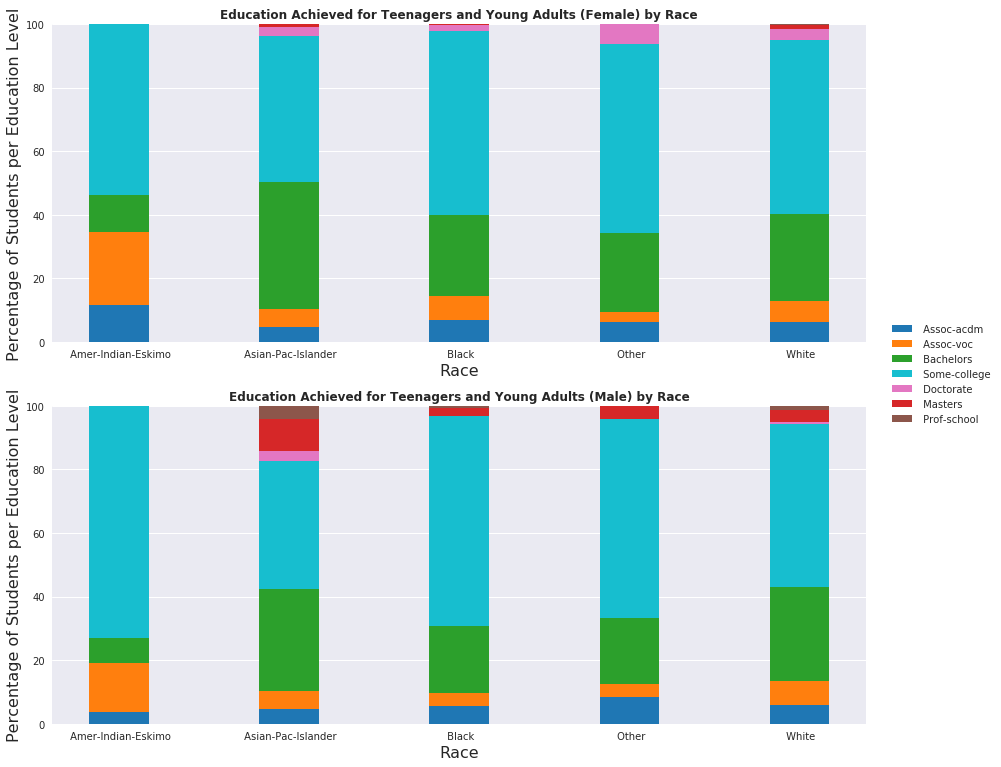
\includegraphics[width=0.5\textwidth]{educationByRace.png}%
  \caption{Education Ages 17-31 By Race and Sex}%
  \label{fig:EducationByRace}%
\end{figure}

One of the biggest dangers in AI is using a Machine Learning model's results questionably. In her work\cite{martin2015ethical}, Kirsten Martin establishes that for Education purposes, beneficial use of data would be to personalize student instruction or identify students at risk of dropping out. Still, questionable use would be to use data for possible admission discrimination. One of our User Stories reflects this bias by using the SHAP Analysis to craft the potential customer that UVW College should focus on, and it was a necessary experience to find value in an Ethical Approach to using Classification Algorithms on data. Great work on the amount of damage that misuse of data is the study Pro Publica did on the COMPAS Recidivism Algorithm\cite{angwin_larson_mattu_kirchner_2016}.

The data shows that more Education leads to more Salary, but that minority groups have a hard time completing their degrees. Additionally, more work hours do not correlate with more Salary, but it raises the question of how to support a student with little to no available time for studies.

We observe that the data is consistent with women having more higher Education than men in Figure~\ref{fig:criticalAgeTarget}. 

\section{Individual Contributions}

My contributions to the project started with building the Jupyter Notebook that loaded the data into a data frame and setup some examples to provide an experimentation sandbox to the team~\ref{pythonPlayground}.

I then proceeded to create Univariate Data Analysis and Multivariate Data Analysis in the form of Whisker BoxPlots, Scatter Plots, and custom made Stacked Bar Charts. I developed all the Stacked Bars in our Report, but my personal favorite was the Education Achieve for Ages 18-30 in Figure~\ref{fig:educationByNationality}. This Visualization shows that all Women from Scotland, Ireland, and Honduras have a doctorate. All Men from Scotland have a Masters's. It was a fun fact mostly because the sample from Scotland is 12 data points in total Ireland 24, and Honduras 13, but it was an exciting find. 

\begin{figure}[!t]
  \centering
  \captionsetup{justification=centering}
  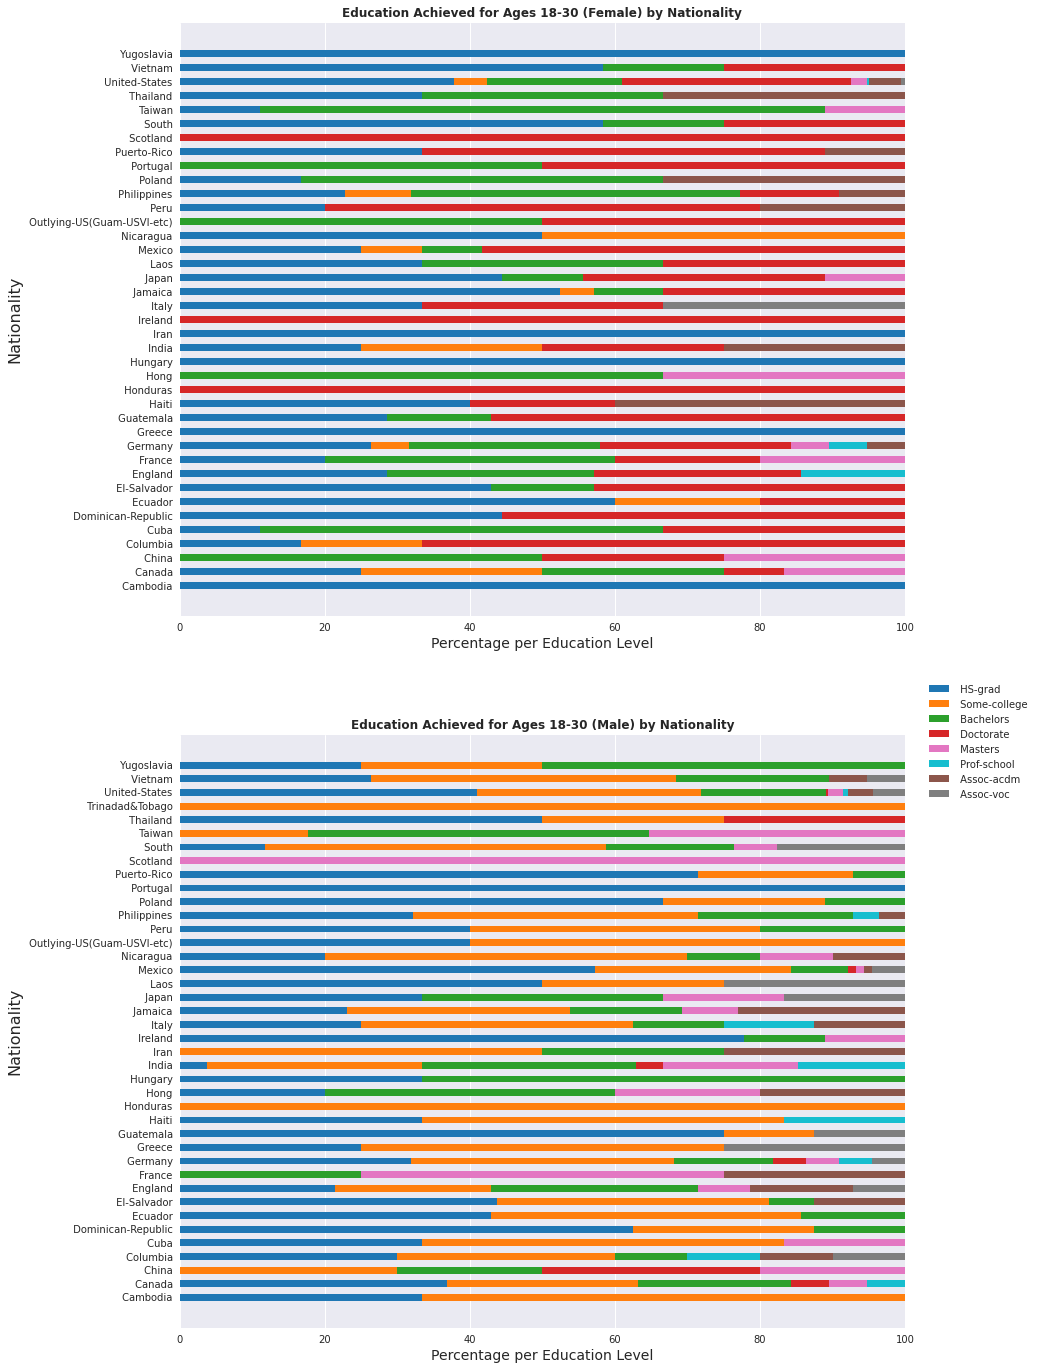
\includegraphics[width=0.5\textwidth]{educationByNationality.png}%
  \caption{Education by Nationality}%
  \label{fig:educationByNationality}%
\end{figure}

While investigating, I also found a few data points on the $<=50K$ class that had Capital Gains visible in Figure~\ref{fig:CapitalGainsAndIncome}, but then I proceeded to plot Capital Gains of 0 in Figure~\ref{fig:ArePeopleWithNoCapitalGainsInOver50KGroup} and found it fascinating. A high number of entries of individuals with no Capital Gains make $<=50K$. 

\begin{figure}[!t]
  \centering
  \captionsetup{justification=centering}
  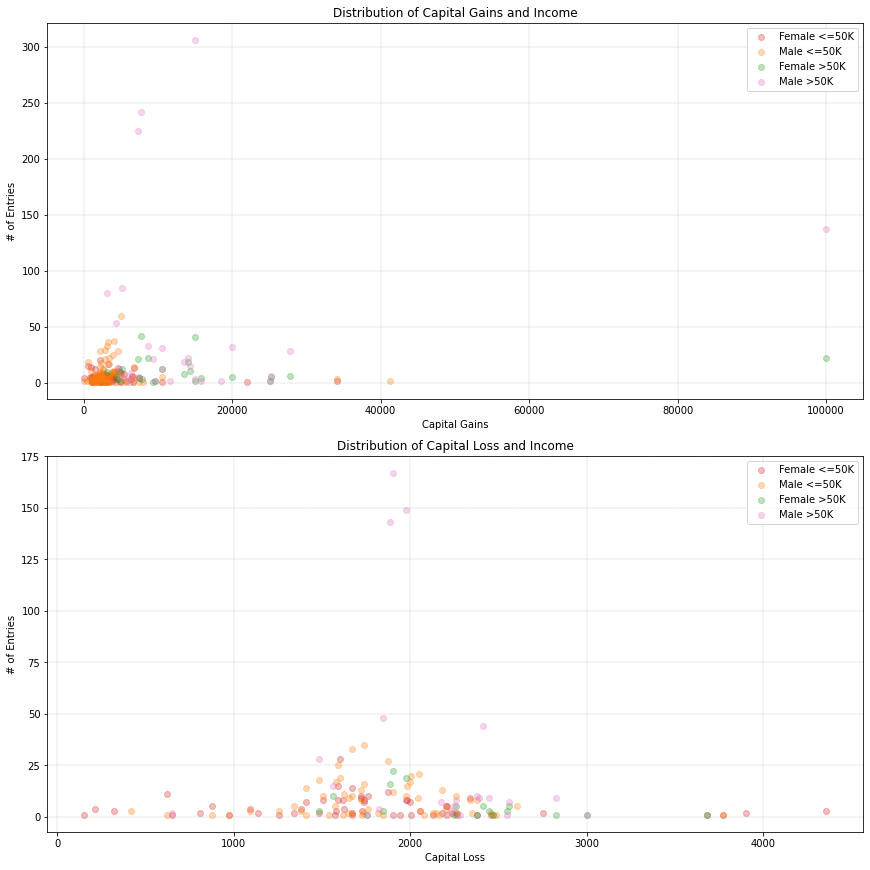
\includegraphics[width=0.5\textwidth]{CapitalGainsAndIncome.png}%
  \caption{Capital Gains and Data Points}%
  \label{fig:CapitalGainsAndIncome}%
\end{figure}

\begin{figure}[!t]
  \centering
  \captionsetup{justification=centering}
  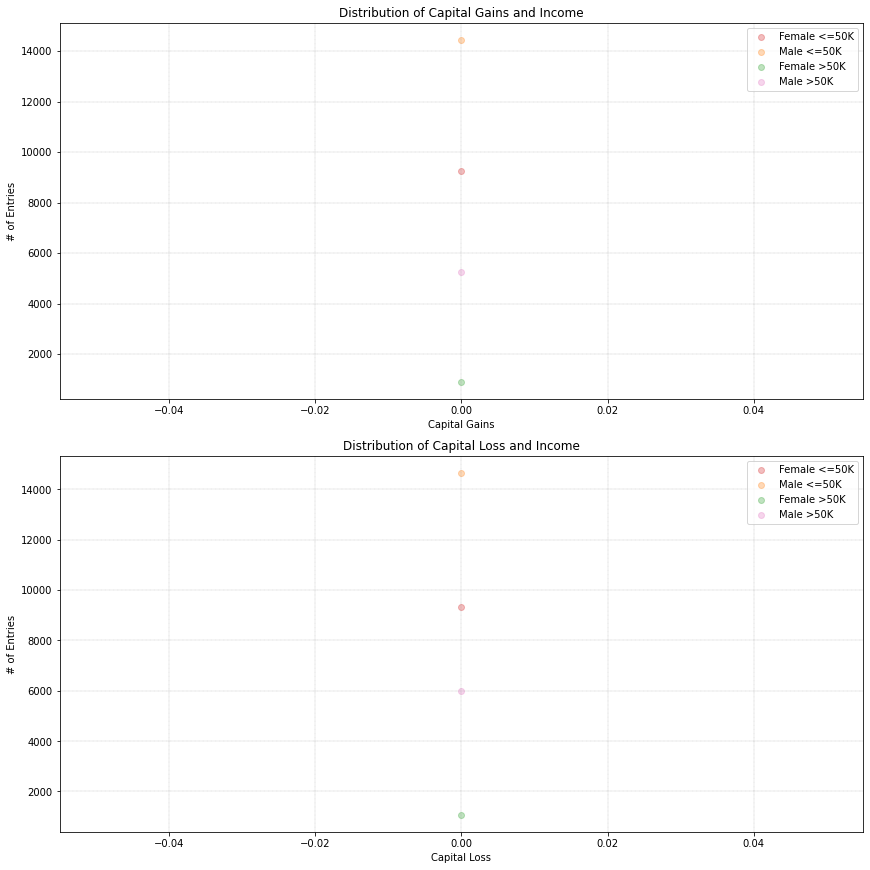
\includegraphics[width=0.5\textwidth]{ArePeopleWithNoCapitalGainsInOver50KGroup.png}%
  \caption{No Capital Gains and Data Points}%
  \label{fig:ArePeopleWithNoCapitalGainsInOver50KGroup}%
\end{figure}

I developed the User Stories we would create for UVW College and started the Systems Documentation Report. Afterward, I proceeded to recruit the team to help with the goal of the project of creating Visualizations to help a Business Team made decisions and reach their conclusions. Each of us developed visualizations for each user story, with the ones mentioned above developed personally. I kept an emphasis on how data can be misleading, and that it is possible to manipulate it to tell a story that is different from what a Business Group would want to discover. 

Another point I focused on is what User Stories would be of interest to UVW College. After a quick investigation on the US Department of Education page on Grants, it clearly shows that there are Grants for a multitude of opportunities\cite{grants}. The existence of so many grants increased the priority of showcasing all minority groups, and segregating the data between male and female, and try to break down groups into more granular demographics were possible.

The SHAP Analysis also showed some influence from the Hours per Week worked, but I quickly dispelled this notion with a simple Scatterplot of the Attribute. The Visualization (Figure~\ref{fig:hoursWorkedVsSalary}) shows that while there are some outliers in the data, it is not enough information to conclude there is a correlation between hours worked and salary earned.

\begin{figure}[!t]
  \centering
  \captionsetup{justification=centering}
  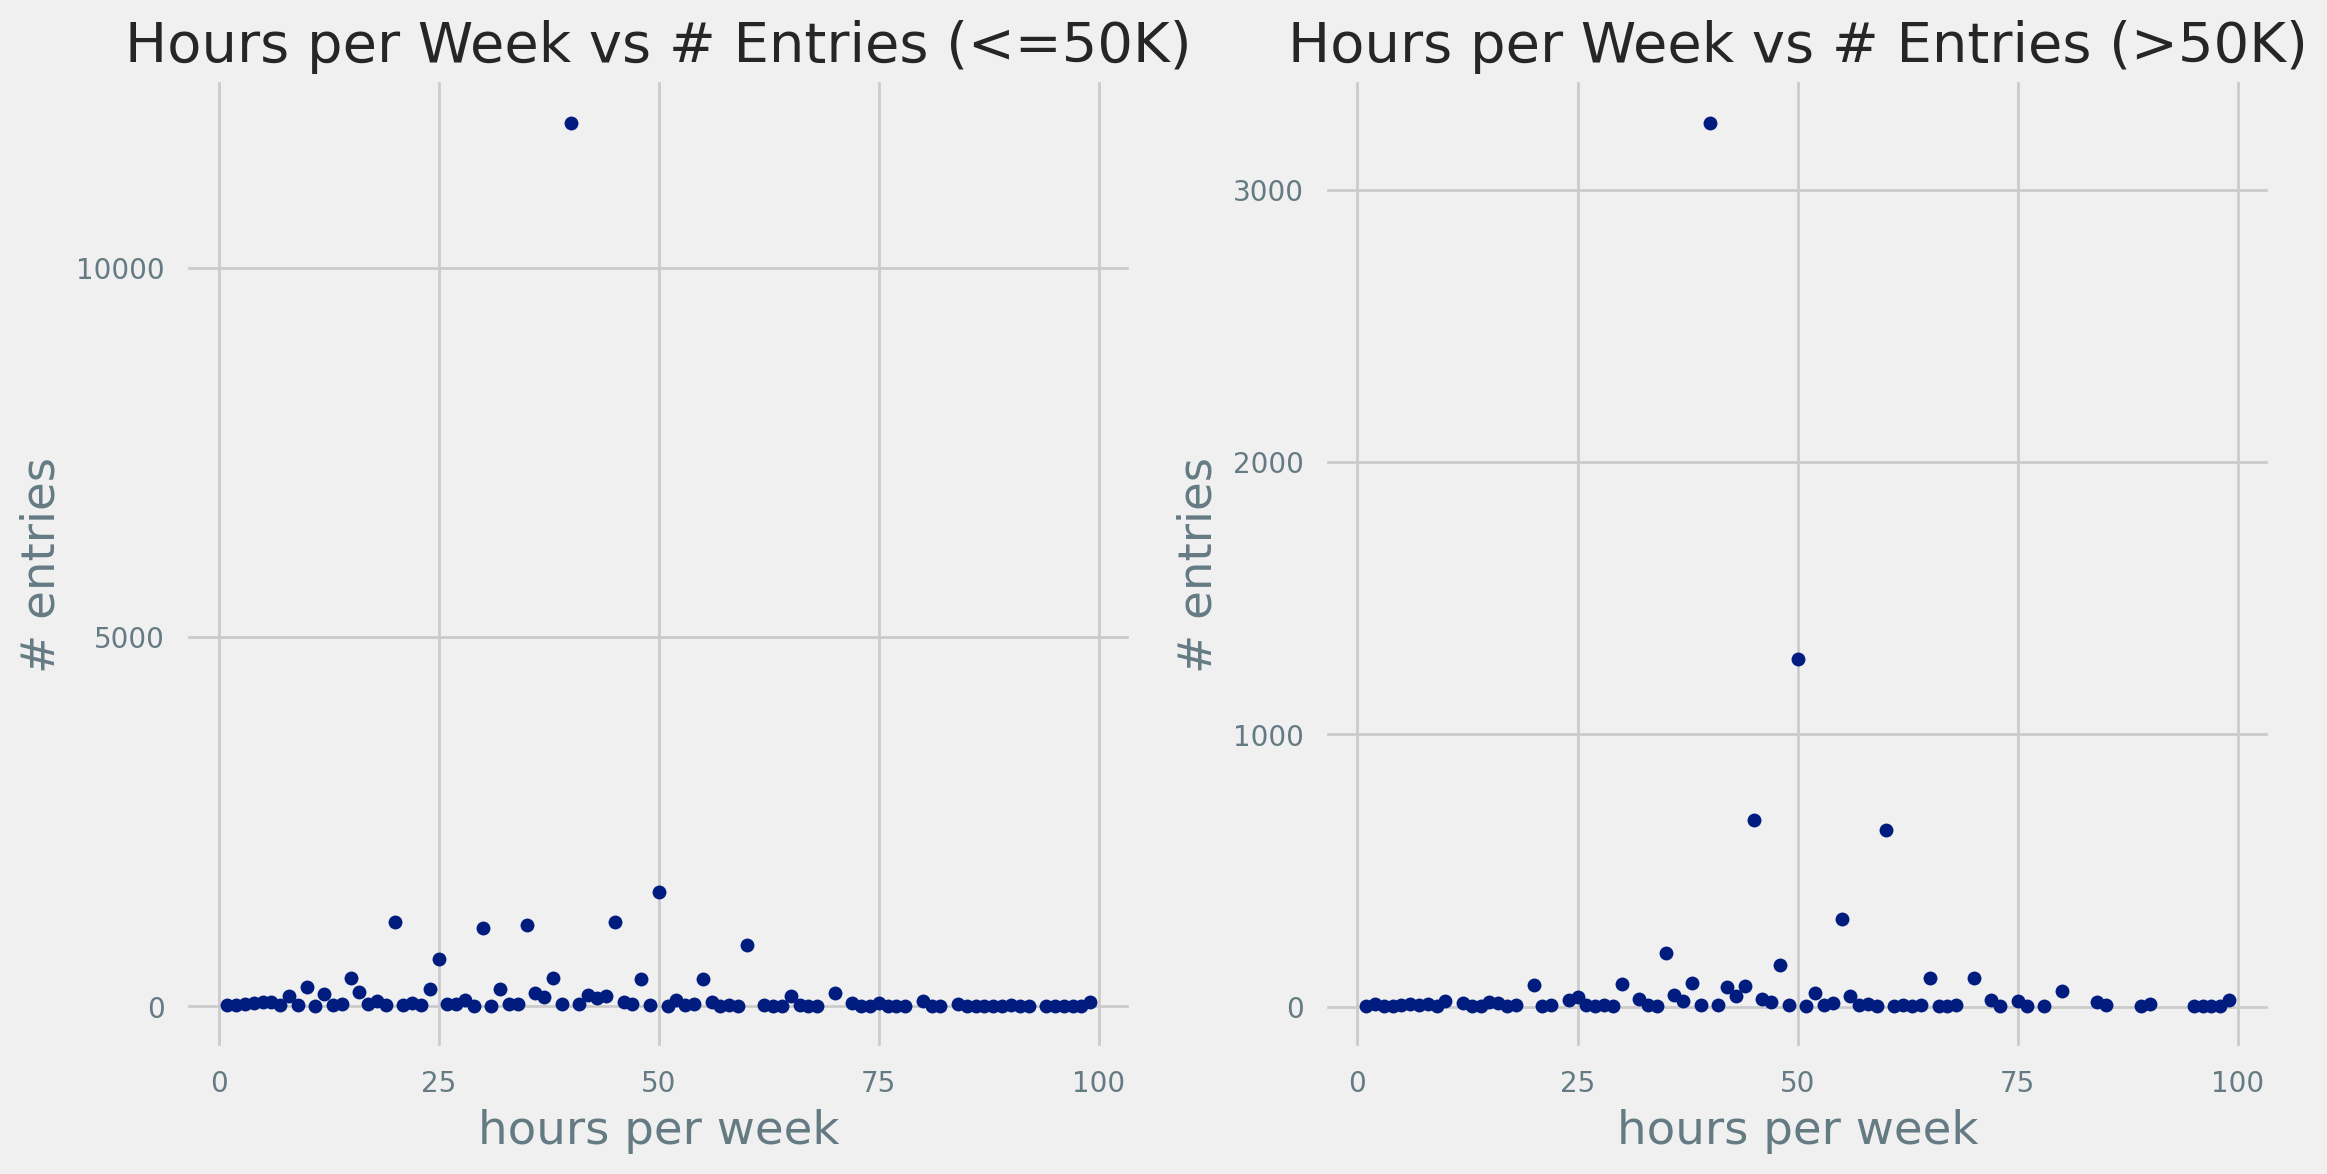
\includegraphics[width=0.5\textwidth]{hoursWorkedVsSalary.png}%
  \caption{Hours Worked vs. Salary}%
  \label{fig:hoursWorkedVsSalary}%
\end{figure}


I set out to find out the critical time that the school should start getting its offerings in front of their potential customers. The expectation was that around 18 people would start to increase in numbers in College Education. This research was also an opportunity to find out when to begin marketing possible Masters or Doctorate programs. I documented Findings in Figure~\ref{fig:criticalAgeTarget}.

\begin{figure}[!t]
  \centering
  \captionsetup{justification=centering}
  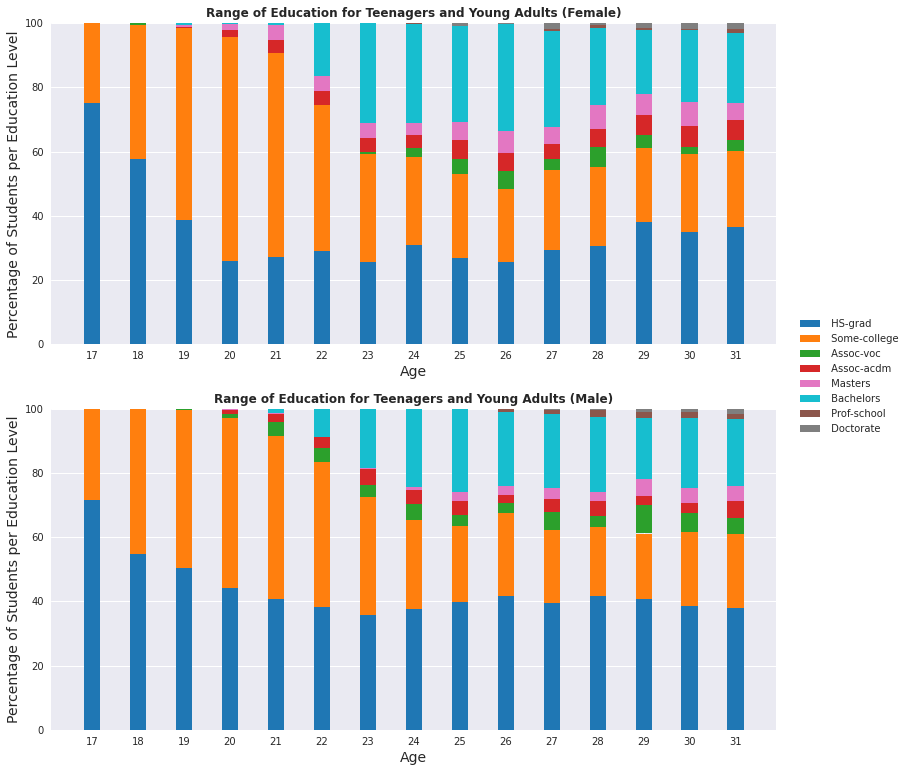
\includegraphics[width=0.5\textwidth]{criticalAgeTarget.png}%
  \caption{Critical Ages to target Marketing Profiles}%
  \label{fig:criticalAgeTarget}%
\end{figure}


\section{Lessons Learned}

The notebook empowered the team to start experimenting with the data. It is something so simple, yet before it was hard to get traction because all individuals in the group were working professionals.

We used the SHAP Analysis in two ways. The first is one where we use the Algorithm to learn more about the data. The second would exploit these biases in an immoral but not unethical approach in which UVW College would only target a specific group of people (White Males that worked in Management). We glossed over a few possible issues while researching data in the course, and it was interesting to see the problems appear in the project.

I focused heavily on using Pandas since I've been using it for a long time, but I always felt like I had a weakness in querying the data. For my Visualizations, I focused on having clear visuals that respected Bertin's Visual Variables. I used Scikit for Normalizing a few values and seaborn for trying out different plots, but I decided to roll out my own Stacked Bar Chart instead.

Working with the team was very beneficial. I learned more about  Scott Lundberg's impressive work with SHapley Additive exPlanations and a CatBoost Classifier.

My main takeaway for the project is observing the biases and issues analyzing data that could happen in the workplace. And how we need a framework to explain to other individuals that data is not to be blindly trusted. By placing a strong faith in the SHAP Analysis and assuming that the data was collected $100\%$ correctly, one might find themselves reaching for the wrong conclusion.

\section{Appendix}

\lstinputlisting[label={pythonPlayground},caption={First few lines of the Sandbox},language=Python, linewidth=\columnwidth,breaklines=true,basicstyle=\small\ttfamily,columns=fullflexible]{./src/example.py}

\bibliographystyle{IEEEtran}
\bibliography{IEEEabrv,cse578}

\end{document}
